%%% 関西大学総合情報学部 松下研究室 中間発表用 TeX テンプレート Ver 1.2 (2015/8/12) %%%

% スタイルファイルは matsushita-zemi.cls を使います
\documentclass[a4j]{matsushita-zemi} 

%図表を使うための設定です
\usepackage[dvipdfmx]{graphicx}
\graphicspath{{./fig/}}
 \usepackage{ascmac}
 \usepackage{framed}

%% タイトル (長くなる場合は\\で適宜改行すること)
\title{中間発表用スタイルファイルの使い方}


%%% 氏名 (姓・名の間は半角スペース) %%%
\idnum{情12-3456}
\author{関大 花子}


% --------------------------------------------------------
\begin{document}
\maketitle

%%% 以下,本文 %%%
\section{はじめに}
\label{background} 

このファイルは,関西大学総合情報学部松下研究室の中間発表用 \LaTeX テン
プレートである.本テンプレートは情報処理学会論文誌ジャーナル用スタイル
ファイルを援用しているため,多くの部分はそれに準拠している.

\section{論文の構成}
\label{works} 

論文の基本構成は以下のようになる.この論文構成は「ものづくり系」の論文
を想定しているが,分析系,実験系の論文も,力点が異なるだけで,これと大
きく外れることはない.


\begin{small}
  \begin{framed}
    \begin{enumerate}

    \item 序論 
      \begin{itemize}
      \item 目的と対象を明示する
      \end{itemize}

    \item 関連研究
      \begin{itemize}
      \item 適切な参考文献(査読付論文,国際会議原稿)を引用する
      \item 多少異なる論文も参考にする
      \item 既存の研究と自分の研究の比較表を作る
      \end{itemize}
      
    \item 提案/デザイン指針
      \begin{itemize}
      \item どのように問題を解決するか
      \item 問題解決の鍵となる考え方は何か
      \item その実現にはどのようなデザインが必要か
      \item どの点について新規性を認められるか
      \end{itemize}
      
    \item 実装
      \begin{itemize}
      \item どのようなプログラム構成か
      \item 他人が再現するのに足る情報提示ができているか
      \end{itemize}
      
    \item 実験
      \begin{itemize}
      \item 実験の統制はどのように行ったか
      \item どのようなデータが得られたか
      \end{itemize}
      
    \item 考察
      \begin{itemize}
      \item どのような分析手法を用いるか
      \item 仮説は検証されたか
      \end{itemize}
      
    \item 結論
      \begin{itemize}
      \item 何が明らかになったか
      \item 何が問題として残されたか
      \end{itemize}
      
    \item 謝辞

    \item 参考文献
    \end{enumerate}
  \end{framed}
\end{small}



\section{論文フォーマットの指針}
\label{sec:format}

以下では,論文フォーマットの指針について述べる.これに従って原稿を執筆
してほしい.なお,\LaTeX を用いた一般的な文章作成技術については,奥村
本\cite{okumura} 等を参考にされたい.


% ------------------------------------------------------------
\subsection{本文}
指摘が不十分な箇所があるかも知れないが,迷ったときは,情報処理学会の
投稿論文に準拠していただくか,先生に問い合わせていただきたい.また,
このファイルは適宜更新し,より合理的かつ理解しやすいフォーマットへと
進化させていきたいと考えているので,諸兄の協力を願う.


% ------------------------------------------------------------
\subsubsection{見出し}

見出しに用いるコマンドは \verb|\section|, \verb|\subsection|, \verb|\subsubsection|
の 3 種類である.原稿執筆の際は,不必要に階層を深くしないよう留意し,
中間発表の原稿では \verb|\subsubsection| の使用はなるべく控えること.

% ------------------------------------------------------------
\subsubsection{行送り}

このスタイルでは 2 段組を採用している.改行は,一行空行を設けることで行
い,原則として段落中では \verb|\\| による改行は行わないこと.ま
た,\verb|\vspace| や\verb|\vskip| を用いたスペースの調整は行わないこ
と.


% ------------------------------------------------------------
\subsubsection{フォントサイズ}

フォントサイズは,スタイルファイルによって自動的に設定されるため,基本
的には著者が自分でフォントサイズを変更する必要はない.なお本文のデフォ
ルトのフォントサイズは 10pt である.


% ------------------------------------------------------------
\subsubsection{句読点}

句点には全角の「.」を,読点には全角の「,」を各々用い,「。」や「、」
は使わないこと.ただし,英文中や数式中で「.」や「,」を使う場合には半角
文字を使うこと (e.g., $[x, y]=[3.1, 2.5]$).括弧と句読点の順には注意し
て欲しい(この文のように括弧の後に句点を打つ).

% ------------------------------------------------------------
\subsubsection{全角文字と半角文字}

全角文字と半角文字の両方にある文字は次のように使い分ける.

\begin{enumerate}
\item 括弧は全角の「(」と「)」を用いる.ただし,書誌データでは半角の
  「(」と「)」を用いる.

\item 英数字,空白,記号類は半角文字を用いる(句読点は除く).

\item カタカナは全角文字を用い,半角は何があっても使わないこと.

\item 引用符では開きと閉じを区別する.開きの引用符には \verb|``|(半角
  の \verb|`| をふたつ)を,閉じの引用符には \verb|''|(半角
  の \verb|'| をふたつ)を各々用いること.
\end{enumerate}

% ------------------------------------------------------------
\subsubsection{箇条書き}

箇条書きを行う場合は,目的に応じて \verb|enumerate| 環境(番号),
\verb|itemize| 環境(丸印),\verb|description| 環境(自分で定義)を各々
用いること.


% ------------------------------------------------------------
\subsubsection{脚注}

脚注は \verb|\footnote| コマンドを使って書くと,ページ単位に脚注が生成される\footnote{脚注の例.}.
なお,ページ内に複数の脚注がある場合,参照記号は \LaTeX を 2 回実行しない
と正しく反映されないので注意すること\footnote{二つ目の脚注.}.
 
また場合によっては,脚注をつけた位置と脚注本体とを別の段に置くほうが良い
こともある.この場合には,\verb|\footnotemark| コマンドや \verb|\footnotetext| コ
マンドを使って対処すること.

% ------------------------------------------------------------
\subsection{数式}\label{sec:Item}

%4.4.1
\subsubsection{本文中の数式}

本文中の数式は \verb|$| と \verb|$|, \verb|\(| と \verb|\)|, あるいは \verb|math| 環境のいず
れで囲んでもよい.

%4.4.2
\subsubsection{別組の数式}

別組数式 (displayed math) については \verb|$| と \verb|$| で囲むのでは
なく,\verb|\[| と \verb|\]| で囲むこと.数式に番号を付与したい場合
は,\verb|equation| 環境(数式が 1 行の場合),あるい
は \verb|eqnarray| 環境(数式が複数行の場合)のいずれかの環境を用いる.
以下に \verb|\[| と \verb|\]| で囲んだ例を示す.
\[
\mathit{div}_{G_i}(d_{jy}) 
\stackrel{\mathrm{def}}{=}\{d_{ix} \in \mathit{gr}(G_i) | d_{ix} \preceq d_{jy}\}
\]


%4.4.3
\subsubsection{eqnarray環境}

互いに関連する別組の数式が 2 行以上連続して現れる場合には,単に
\verb|\[| と \verb|\]|,あるい は \verb|\begin{equation}|
と \verb|\end{equation}| で囲った数式を書き並べるのではなく,
\verb|\begin|\allowbreak\verb|{eqnarray}| と \verb|\end{eqnarray}| 
を使って,等号(あるいは不等号)の位置で縦揃えを行なった方が読みやすい.
以下に \verb|eqnarray| 環境の例を示す.イコールの位置で揃っていることに注目.
%
\begin{eqnarray}
\Delta_l &=& \sum_{i=l|_1}^L\frac{\delta_{i}}{\Psi }\\
\frac{\partial y}{\partial x} &=& e^{-ax} \Bigl\{ \int e^{ax} Q(x)dx + C\Bigl\}
\end{eqnarray}
%

%4.5
\newpage
\subsection{図}

1段の幅におさまる図は,図\ref{fig:single} の形式で指定する.このとき,
位置の指定に \verb|[h]| オプションは使わない.

\begin{figure}[tb]
  \centering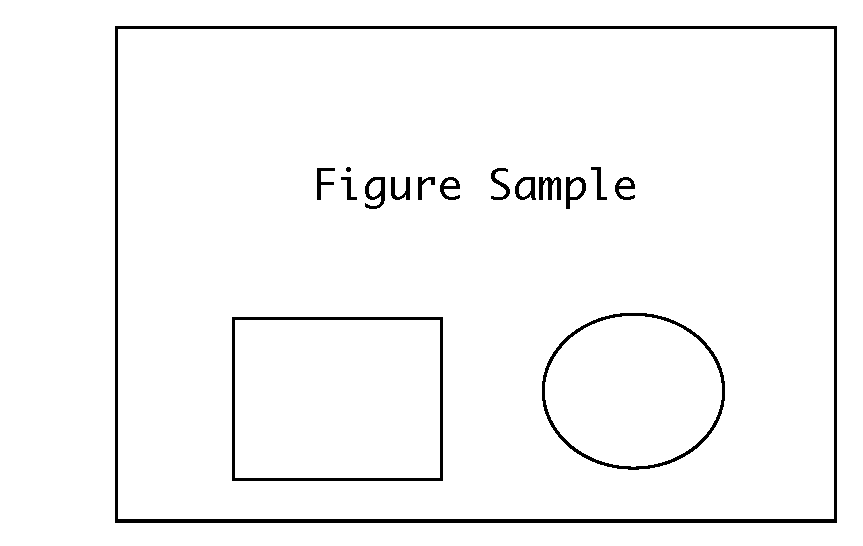
\includegraphics[clip, width=.95\columnwidth]{figureSample.eps}
  \caption{1段幅の図のサンプル}
  \label{fig:single}
\end{figure}


\begin{figure}[t]
  \begin{minipage}{0.49\hsize}
    \begin{center}
      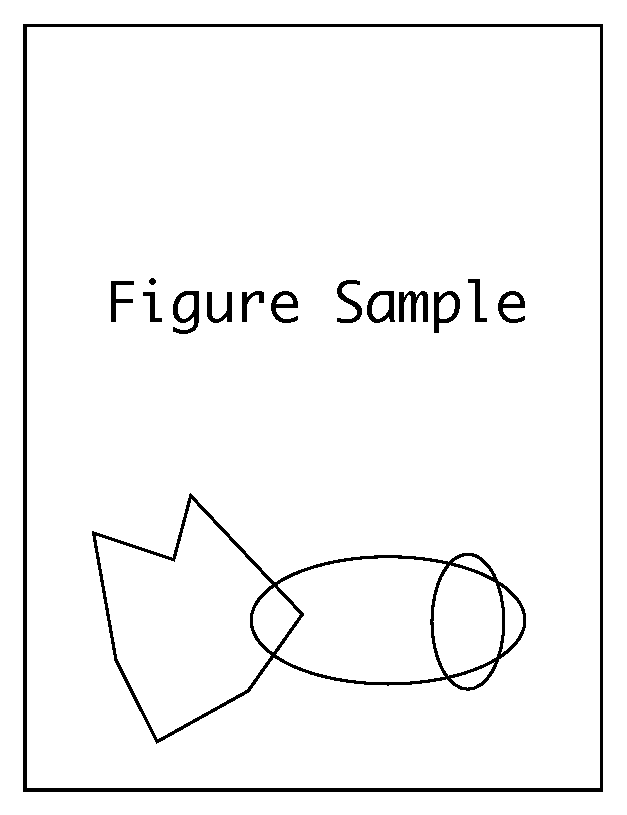
\includegraphics[clip, width=.8\textwidth]{figureSample2.eps}\\
      \small{(a) 右図}
    \end{center}
  \end{minipage}%
  \begin{minipage}{0.49\hsize}
    \begin{center}
      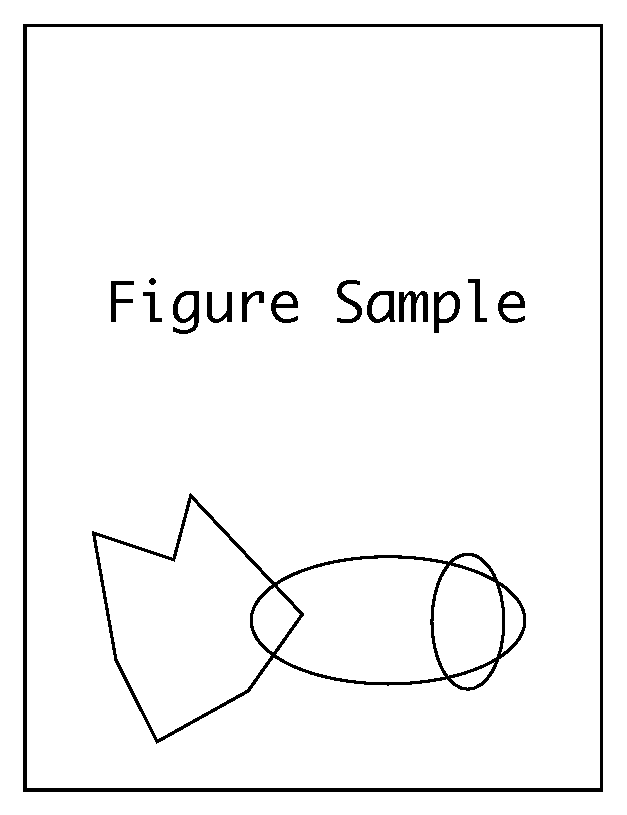
\includegraphics[clip, width=.8\textwidth]{figureSample2.eps}\\
      \small{(a) 左図}
    \end{center}
  \end{minipage}
  \vspace{2pt}
  \caption{並べた図のサンプル}
  \label{fig:twoGraphs}
\end{figure}


\begin{figure*}[tb]
  \centering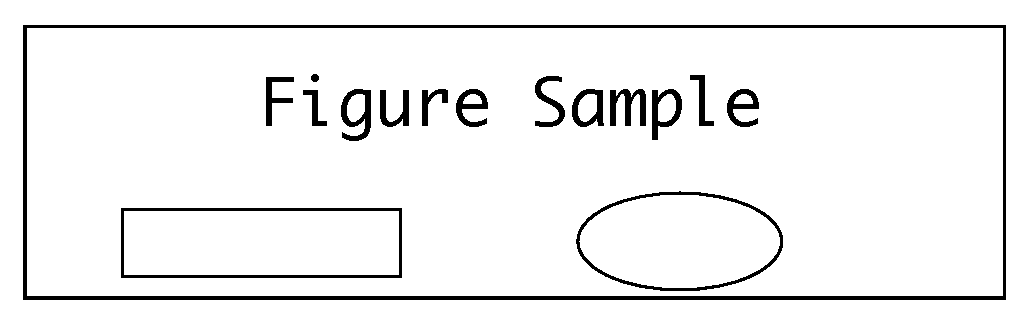
\includegraphics[clip, width=.9\textwidth]{figureSample3.eps}
  \caption{2段幅の図のサンプル}
  \label{fig:double}
\end{figure*}


またひとつの図のなかに複数の図を並べて表示したい場合には,\verb|minipage|
環境を使って,図\ref{fig:twoGraphs} のようにすることで実現できる.

2 段の幅にまたがる図は,図\ref{fig:double} の形式で指定する.
位置指定のオプションは \verb|[t]| しか使えない.

図の中身では本文と違い,どのような大きさのフォントを使用しても構わない
が,刷り上がり時に読めるサイズであることに留意すること.図の中身とし
て,encapsulate されたPostScriptファイル(いわゆるEPSファイル)を読み込
むことができる.mac\TeX の場合は読み込みには,プリアンブルで
%
\begin{framed}
    \verb|\usepackage[dvipdfmx]{graphicx}|
\end{framed}
%

\noindent
を行った上で,\verb|\includegraphics| コマンドを図を埋め込む箇所に置き,
その引数にファイル名(など)を指定する.Windows\TeX の場合
は,\verb|[dvipdfmx]| のところを\verb|[dviout]|というオプションに変更す
ること.

%4.6
\subsection{表}

表の罫線はなるべく少なくするのが,仕上がりをすっきりさせるコツである.
罫線をつける場合には,一番上の罫線には二重線を使い,左右の端には縦の罫
線をつけない(表\ref{tab:example}).また,見出し(\verb|\caption|)は,
表の場合は図と違って上側であるので注意していただきたい.

\begin{table}[tb] 
  \caption{表の例} 
  \label{tab:example}
  \hbox to\hsize{\hfil
    \begin{tabular}{l|lll}
      \hline\hline
           & column1     & column2  & column3 \\
      \hline
      row1 &	item 1,1 & item 2,1 & ---\\
      row2 &	---      & item 2,2 & item 3,2 \\
      row3 &	item 1,3 & item 2,3 & item 3,3 \\
      row4 &	item 1,4 & item 2,4 & item 3,4 \\
      \hline
    \end{tabular}\hfil}
\end{table}

%4.7
\subsection{参考文献・謝辞}

参考文献は \verb|.bib| ファイルに記述し,\BibTeX でコンパイルする方法を
推奨する.

%4.7.1
\subsubsection{参考文献の参照}

本文中で参考文献を参照する場合には \verb|\cite| を使用する.参照されたラ
ベルは自動的にソートされ番号が付与される.

\begin{framed}
文献 \verb|\cite{okumura, companion}| は \LaTeX の総合的な解説書である.
\end{framed}
\noindent
と書くと,
\begin{framed}
文献\cite{okumura, companion}は \LaTeX の総合的な解説書である.
\end{framed}
\noindent
が得られる.

%4.7.2
\subsubsection{参考文献リスト}

参考文献リストには,原則として本文中で引用した文献のみを列挙する.順序
は参照順あるいは第一著者の苗字のアルファベット順とする.文献リスト
は\BibTeX と\verb|matsort.bst|(アルファベット順)を用いて作
り,\verb|\bibliograhpystyle| と \verb |\bibliography| コマンドにより利
用することができる.これらを用いれば,規定の体裁にあったものができるの
で,できるだけ利用していただきたい.何らかの理由で thebibliography 環境
で文献リストを「手作り」しなければならない場合は,できるところま
で \BibTeX で作り,でき上がった \verb|.bbl| ファイルを加工すると工数が
減り効率的である(人工知能学会全国大会などオンライン予稿集の場合がそれ
に相当する).

\subsubsection{参考文献のタイプ}

詳細は,\verb|bibsample.bib| を参照されたい.卒業論文や修士論文で主に使
われるのは,書籍用の \verb|@Book|(e.g., \cite{okumura,companion}),原
著論文用の \verb|@article|(e.g., \cite{j024, j027}),国際会議予稿集用
の\verb|@inproceedings|(e.g., \cite{c028})である.なお,国内の全国大
会,研究会は基本的に国際会議と同様に\verb|@inproceedings|を用いること
(e.g., \cite{m139, m174}).なお,人工知能学会のように,オンラインプロ
シーディングスしかない場合はページの代わりに,発表番号
を \verb|presentation| のところに書く(e.g., \cite{m186}).詳細
は \verb|bibsample.bib|中のエントリ \verb|m186| を参照のこと.


%4.7.3
\subsubsection{謝辞}

謝辞がある場合には,参考文献リストの直前に,\verb|\section*{謝辞}| とい
う章を設けて記述する.科研費を始めとする外部予算を受けている場合は,必
ずここに研究費に対する謝辞「本研究は日本学術振興会科学研究費補助金基盤
研究(x)(課題番号:xxxxxx)の支援により実施された.」のように記述する
こと.


\section*{謝辞}
本テンプレートは情報処理学会の投稿論文フォーマットを参考にしている.記
して謝意を表す.


%%% 参考文献 %%%
\bibliographystyle{matsort}
\bibliography{bibsample.bib}

\end{document}